\chapter{Panel administratora}

\section{Logowanie do panelu administratora}
W poniższej sekcji przedstawiony zostanie proces logowania do panelu administratora w aplikacji. W pierwszej kolejności użytkownik musi wybrać opcję \textit{Rozpocznij}, dostępną z~ poziomu górnego menu na stronie głównej, a następnie wybrać przycisk \textit{Logowanie z~ Google}. Poniższy rysunek \ref{Rys:logowanieee} przedstawia okno logowania administratora.

\begin{figure}[h]
	\centering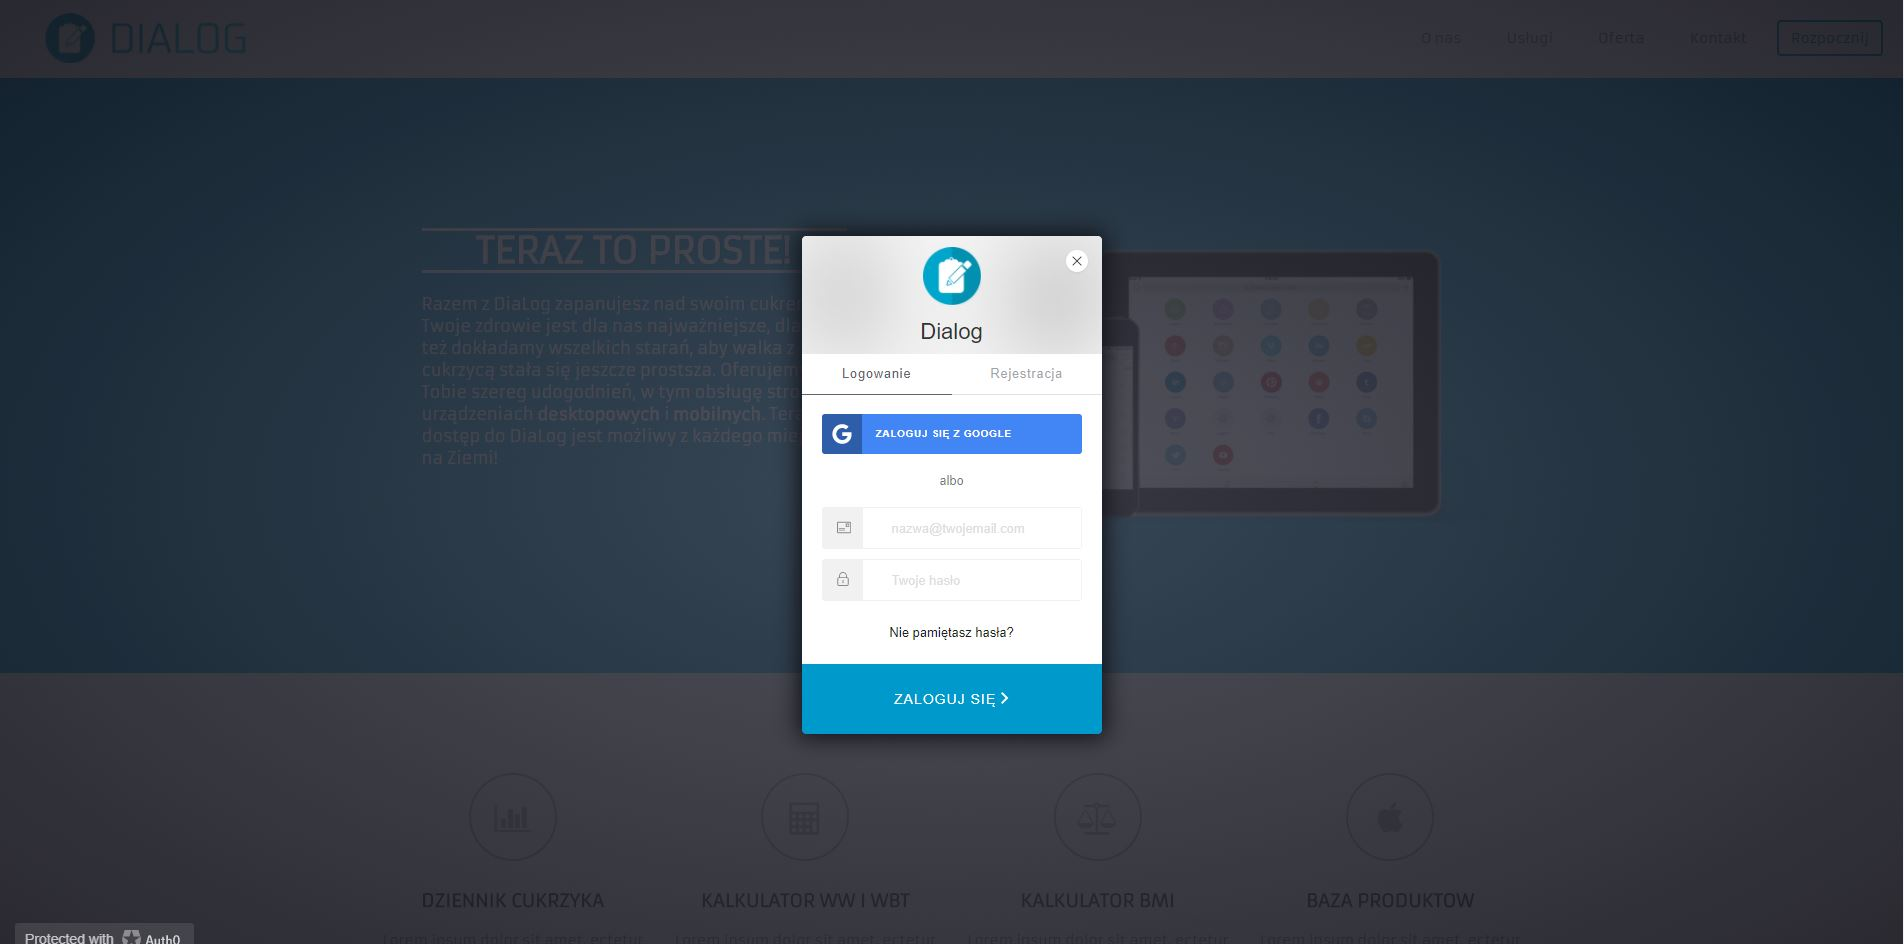
\includegraphics[scale=0.3]{images/logowanie_google.jpg}
	\caption{Okno logowania administratora}
	\label{Rys:logowanieee}
\end{figure}

Po wybraniu przycisku \textit{Logowanie z Google} należy zalogować się na konto z przypisanymi uprawnieniami administracyjnymi. Pojawi się wówczas dodatkowa pozycja w menu górnym -- \textit{Admin}, co przedstawione zostało na rysunku \ref{Rys:ekran_admin}.

\newpage

\begin{figure}[h]
	\centering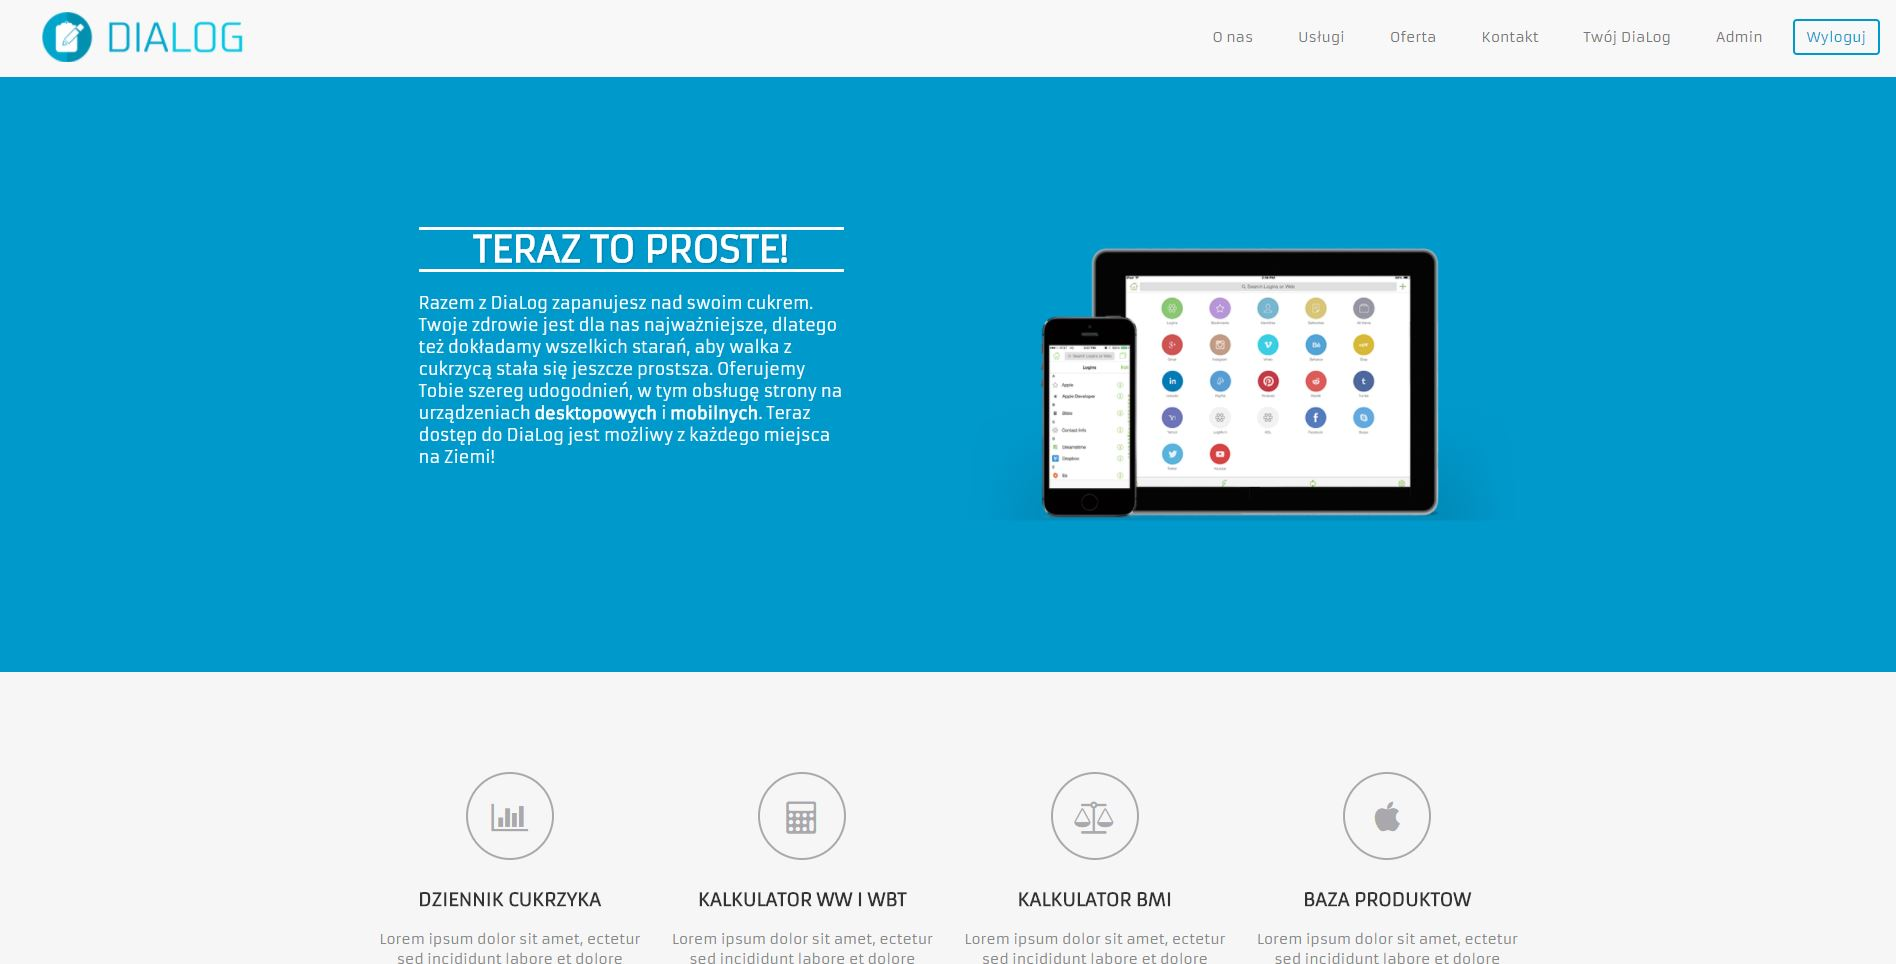
\includegraphics[scale=0.3]{images/ekran_admin.jpg}
	\caption{Okno główne aplikacji z dostępną opcją panelu administratora}
	\label{Rys:ekran_admin}
\end{figure}

\section{Użytkowanie panelu administratora}
Po kliknięciu przycisku \textit{Admin} użytkownik uzyskuje dostęp do Panelu Administratora. Panel ten został stworzony wyłącznie po to, aby usuwać błędnie dodane, bądź zduplikowane produkty dodane do bazy danych produktów. Jest to niezbędny element w przypadku funkcjonalności danej aplikacji rozszerzanych przez użytkowników. Dzięki takiemu rozwiązaniu Administrator w prosty sposób może kontrolować treść zawartą na stronie i~ w razie potrzeby usuwać ją. Panel administratora przedstawiony został na rysunku   \ref{Rys:panel_admin}. Panel został zaprojektowany w postaci tabeli tak, aby w prosty i przejrzysty sposób zaprezentować wszystkie dostępne dane. Ponieważ baza produktów może być stale rozszerzana, a ich ilość może sięgać nawet kilkuset elementów, zastosowana została paginacja tabeli, dzieląca jej zawartość na strony zawierające po dziesięć elementów.


\begin{figure}[h]
	\centering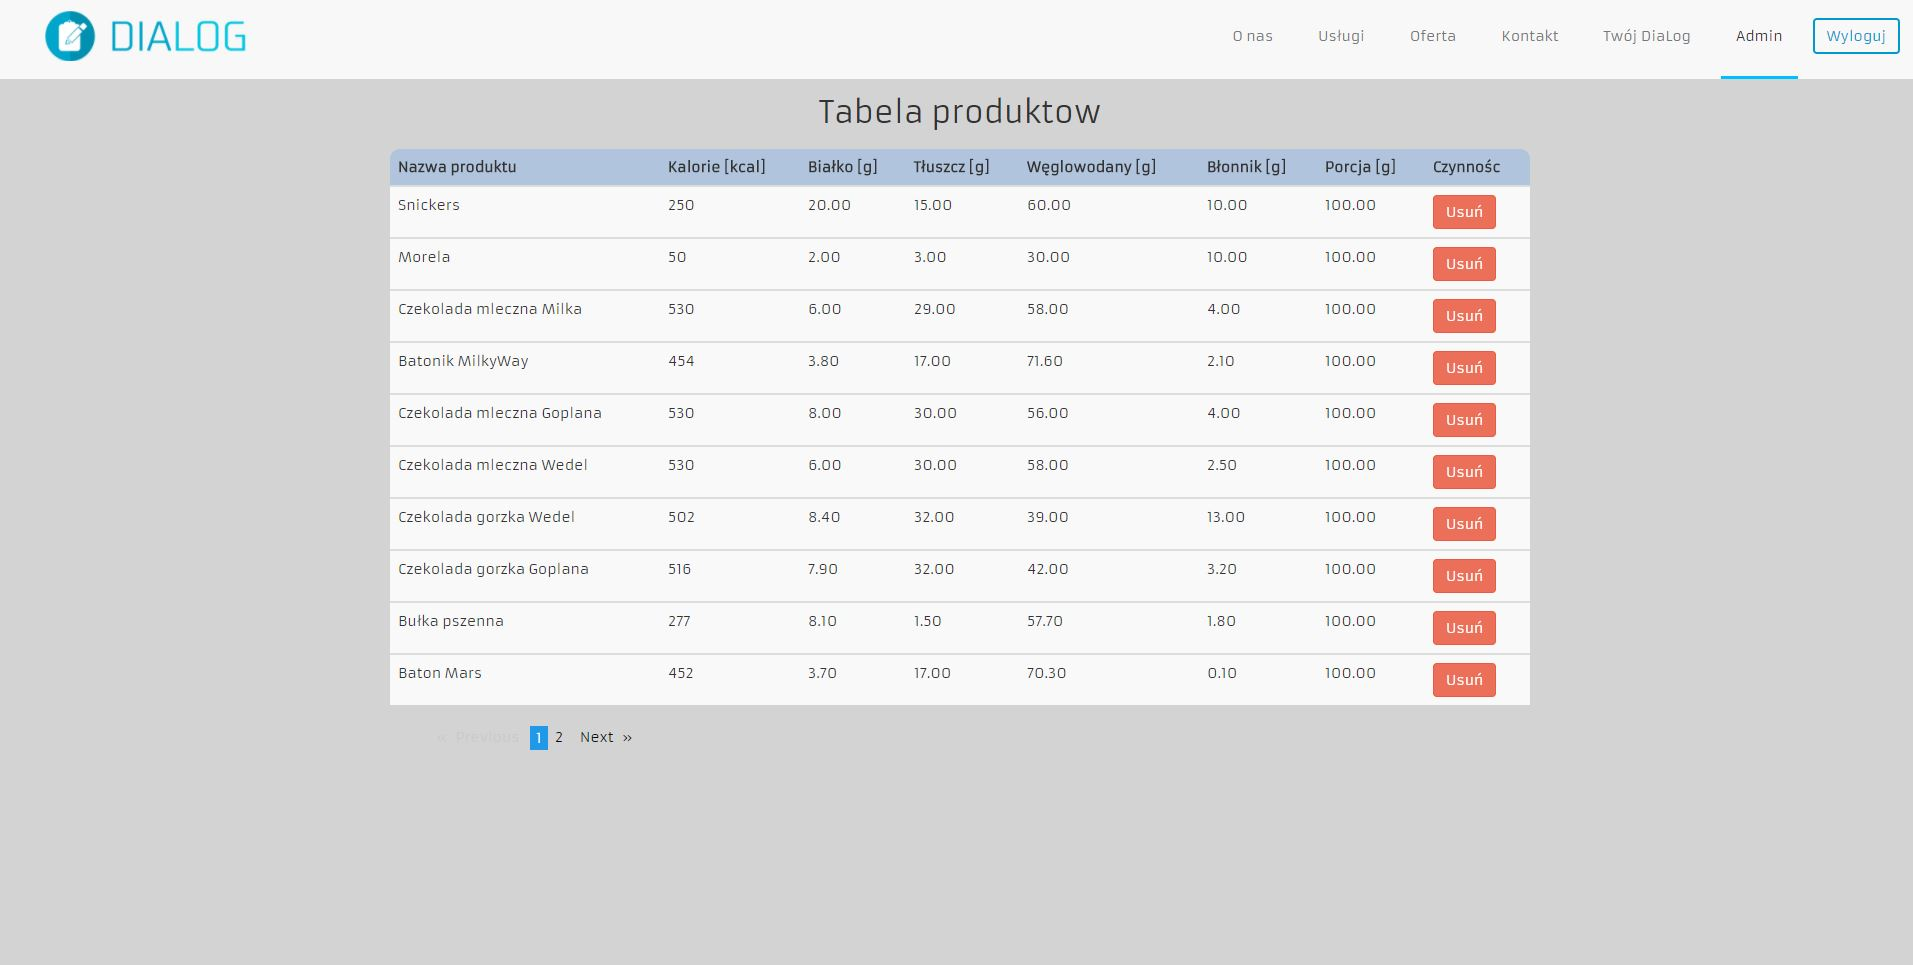
\includegraphics[scale=0.3]{images/panel_admin.jpg}
	\caption{Panel administratora aplikacji}
	\label{Rys:panel_admin}
\end{figure}

Tabela podzielona jest na osiem kolumn:
\begin{enumerate}
	\item \textit{Nazwa produktu},
	\item \textit{Kalorie [kcal]},
	\item \textit{Białko [g]},
	\item \textit{Tłuszcz [g]},
	\item \textit{Węglowodany [g]},
	\item \textit{Błonnik [g]},
	\item \textit{Porcja [g]},
	\item \textit{Czynność}.
\end{enumerate}

W kolumnie \textit{Czynność} przy każdym z wierszy dostępny jest przycisk \textit{Usuń}, dzięki któremu Administrator może usunąć wybrany produkt. Usuwanie produktu odbywa się w~ sposób dynamiczny, co oznacza, że produkt po usunięciu od razu (bez odświeżenia strony) znika z listy dostępnych produktów i nie jest on dostępny nawet z poziomu tabeli produktów dostępnej w zakładce \textit{Kalkulatory} z poziomu panelu użytkownika zalogowanego. 

Administrator, tak jak każdy zalogowany użytkownik, ma również możliwość korzystania ze wszystkich funkcjonalności systemu przeznaczonych dla tej grupy użytkowników -- zakładka \textit{Twój DiaLog}.

